\documentclass{article}


\usepackage{arxiv}

\usepackage[utf8]{inputenc} % allow utf-8 input
\usepackage[T1]{fontenc}    % use 8-bit T1 fonts
\usepackage{hyperref}       % hyperlinks
\usepackage{url}            % simple URL typesetting
\usepackage{booktabs}       % professional-quality tables
\usepackage{amsfonts}       % blackboard math symbols
\usepackage{nicefrac}       % compact symbols for 1/2, etc.
\usepackage{microtype}      % microtypography
\usepackage{lipsum}
\usepackage{amsmath}
\usepackage{graphicx}
\usepackage{wrapfig}

\title{Deep Kalman Filters}


\author{
    Nikita Chizhov \\
    Skolkovo Institute of Science and Technology\\
    \texttt{Nikita.Chizhov@skoltech.ru} \\
   \And
    Ekaterina Ivanova \\
    Skolkovo Institute of Science and Technology\\
    \texttt{Ekaterina.Ivanova@skoltech.ru} \\
  \And
    Vadim Liventsev \\
    Skolkovo Institute of Science and Technology\\
    \texttt{Vadim.Liventsev@skoltech.ru} \\
}

\begin{document}
\maketitle


\keywords{Kalman Filter \and Deep learning \and Bayesian methods}


\section{Introduction}
In Deep Kalman Filters, Krishnan et al. attempt to apply a modified version of Kalman Filters to determine what the best course of treatment for a patient might be, even for patients with only an incomplete medical history. Kalman filters are generative probabilistic graphical models for time series data. Despite the broad success of Kalman Filters, they are limited in their ability to model complex sequential data due to their assumptions of linear relationships between successive latent states and between latent states and observed states. Extention of classical Kalman Filters by replacing linear transformations with nonlinear transformations parameterized by neural networks, is proposed in ``Deep Kalman Filters'' \cite{krishnan2015deep}.The technique was applied to perturbed MNIST data, which the authors refer to as a "Healing MNIST database".

\section{Background}

The classical Kalman Filter aims to model latent states $\vec{z} = (z_1, \dots, z_T)$, $x_t\in\mathbb{R}^s$, using a sequence of observations $\vec{x} = (x_1, \dots, x_T)$, $x_t\in\mathbb{R}^d$ and actions $\vec{u} = (u_1, \dots, u_{T-1})$, $x_t\in\mathbb{R}^c$, as follows:

\begin{equation}
z_t =\mathcal{N}(G_tz_{t-1} + B_tu_{t-1} + \epsilon_t ~ \text{(action-transition)}, \qquad
x_t=F_tz_t + \eta_t ~ \text{(observation)}
\end{equation}

\section{Model}
The authors propose to change all the linear functions the Kalman filter modeling to be neural networks. Suppose that we have unobserved latent variables $\vec{z} = (z_1, \dots, z_T)$ and corresponding observations $\vec{x} = (x_1, \dots, x_T)$, $x_t\in\mathbb{R}^d$ and actions $\vec{u} = (u_1, \dots, u_{T-1})$, $x_t\in\mathbb{R}^c$,  $x_t\in\mathbb{R}^s$. We assume the observations are a noisy, non-linear function of this latent state. We also assume that we can observe actions, which affect the latent state in a
non-linear manner.

The generative model for the deep Kalman filter is then given by:

\begin{equation}
\begin{gathered}
z_1 \sim \mathcal{N}(\mu_0; \Sigma_0) \\
z_t \sim \mathcal{N}(G_{\alpha}(z_{t-1},u_{t-1}, \delta_t),S_{\beta}(z_{t-1},u_{t-1}, \delta_t))\\
x_t \sim \Pi(F_{\kappa}(z_t)). 
\end{gathered}
\end{equation}

The observations $x_t$ are distributed according to a distribution $\Pi$ - a Bernoulli distribution if the data is binary, whose parameters are a function of the corresponding latent state $z_t$.
The functions $G_{\alpha}; S_{\beta}; F_{\kappa}$ are assumed to be parameterized
by deep neural networks. We set $\mu_0 = 0, \Sigma_0 = I_d$.

\subsection{ELBO maximization}
\label{sec:elbo}
Our training step involves optimizing our choices of $F, G$, and $B$ such that they maximize the conditional log-likelihood $\max_\theta\log p_\theta(x)$ for a generative model. This can be done tractably, if not analytically, for linear transformations. However, non-linear transformations render the posterior distribution $p_\theta(\vec{z} | \vec{x}, \vec{z})$ intractable to compute. In order to overcome the intractability of posterior inference, we make use of variational autoencoders. The key concept is that an approximation $q_\phi$ of the posterior is trained using a recognition network. 

We want to maximize the lower bound $\mathcal{L}(x;(\phi, \theta))$ in the following equation using stochastic backpropagation:

\begin{gather*}
\log p_\theta(\vec{x}|\vec{z}) \geq \mathcal{L}(x;(\phi, \theta)) = \\
\sum\limits_{t=1}^{T}\mathbb{E}_{q_\phi(z_t|\vec{x}, \vec{z})}[p_\theta(x_t|z_t)] - KL(q_\phi(z_1|\vec{x}, \vec{z})||p_0(z_1)) - \\
\sum\limits_{t=2}^{T}\mathbb{E}_{q_\phi(z_{t-1}|\vec{x}, \vec{z})}KL(q_\phi(z_t|z_{t-1},\vec{x}, \vec{z})||p_0((z_t|z_{t-1}, u_{t-1}))
\end{gather*}

ELBO is differentiable in the parameters of the model $(\phi; \theta)$, and we can apply backpropagation for updating $\theta$, and stochastic backpropagation for estimating the gradient w.r.t. $\phi$ of the expectation terms w.r.t. $q_\phi(z_t)$. Since we can use Monte Carlo estimates of the gradients of $\mathbb{E}_{q_\phi(z_t|\vec{x}, \vec{z})}[p_\theta(x_t|z_t)]$ and $KL(q_\phi(z_1|\vec{x}, \vec{z})||p_0(z_1))$ w.r.t. $q_\phi(z_t)$, we can use stochastic back-propagation in a variational autoencoder whose objective is to maximize the lower bound using an inference-update algorithm (fig.\ref{fig:alg}).. 

\begin{figure}[h]
\centering
\includegraphics[width=0.5\textwidth]{alg.png}
\caption{Algorithm for learning DKF}
\label{fig:alg}
\end{figure}

In this work we use several types of recognition network, which were proposed by the authors. They consider four variational models: two multi-layer perceptron
and two neural network models. 

\begin{itemize}
   \item \emph{q-INDEP}: $q(z_t |x_t , u_t )$ parameterized by an MLP
   \item \emph{q-LR}: $q(z_t |x_{t-1} , x_t , x_{t+1} , u_{t-1} , u_t , u_{t+1]} ) $ parameterized by an MLP
   \item \emph{q-RNN}: $q(z_t |x_1 , \dots , x_t , u_1 , \dots u_t )$ parameterized by a RNN
   \item \emph{q-BRNN}: $q(z_t |x_1 , \dots , x_T , u_1 , \dots , u_T )$ parameterized by a bi-directional RNN
\end{itemize}


\section{Experiments}

\subsection{Dataset}

In our project we tried to reproduce the original dataset used in the paper. Authors called synthetic dataset “Healing MNIST”. To create this dataset, we used images from the original MNIST
dataset and subjected them to step by step transformations (rotations), as well as bit flipping with 15\%, to obtain a sequence of transformations of the same image. We also added  superimposed an image over the top left corner of three consecutive transformations as it was proposed in original paper. 
We made experiments on several versions of created dataset. The first one consists of sequences of transformations of images of all digits, and the smaller one, which contains sequences of transformations of images of only one digit 1. There were 60000 and 6000 sequences respectively in each dataset.

\begin{figure}[h]
\centering
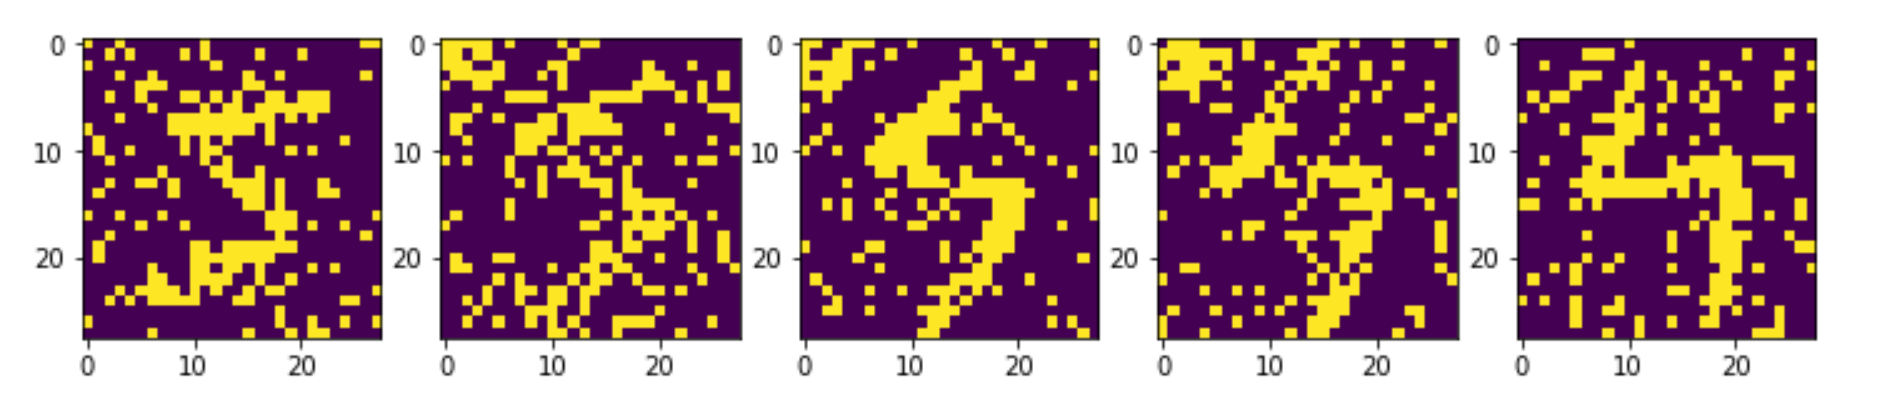
\includegraphics[width=0.7\textwidth]{mnist.png}
\caption{Healing MNIST}
\label{fig:data}
\end{figure}



\subsection{Model variations}

Due to a number of details being ommited in the original paper we experimented with different options for filling these blanks. We tried:

Representing $ G_{\alpha} $ as:

\begin{itemize}
\item MLP with 1, 2, 3, 4, 5 layers with ReLU nonlinearity
\item 1 and 2 layered GRU (with $ z_{t-1} $ as hidden state and $ u_{t-1} $ as input) 
\item 1 and 2 layered LSTM (with $ z_{t-1} $ as a concatenation of hidden state and cell state and $ u_{t-1} $ as input). We tried hidden layer sizes 784 (the size of an inout image), 500, 200, and 80
\end{itemize}

Representing $ F_{\kappa} $ as MLP with 1, 2, 3, 4, 5 with ReLU nonlinearity and sigmoid on top of the last layer

We implemented 2 variational models (see section \ref{sec:elbo}) $q(z|x,u)$: 
\begin{enumerate}
    \item $ q_{\text{INDEP}} (z_t|x_t,u_t)$, parametrized with a 5-layer fully connected neural network with ReLU or Tanh (we tried both) $Q(x,u)$
    \item $ q_{\text{RNN}}(z_t|x, u) $, parametrized with a Recurrent Neural Network $Q(x,u)$
\end{enumerate}

The best reconstruction of MNIST via any of those models is the following:

\begin{figure}[h]
\centering
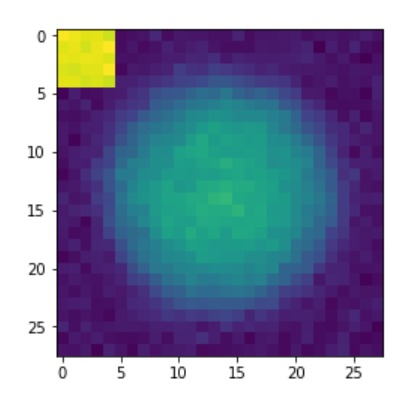
\includegraphics[width=0.4\textwidth]{best_reconstr.jpg}
\caption{Best reconstruction with Deep Kalman Filters}
\label{fig:rec}
\end{figure}

\section{Training procedure}

In the \emph{forward pass} we 
\begin{enumerate}
    \item Sample a batch of images $x$ and actions $u$ from the dataset
    \item Calculate the mean of $q(z|x,u)$ using $Q(x,u)$
    \item Draw a sample from the standard normal distribution and multiply by mean and variance of $q(z|x,u)$ to obtain sample $z$ (reparametrization trick)
    \item Apply $G_{\alpha}(z_t)$ to $z_1,z_2,\dots,z_{n-1}$ to obtain $\hat{z_2},\hat{z_3},\dots,\hat{z_n}$
    \item Calculate ELBO using the formula from section \ref{sec:elbo}
\end{enumerate}

In the \emph{backward pass} we use Pytorch to backpropagate ELBO through our entire model and make an update to the model parameters using Adam optimizer with learning rate 0.001.

\section{Baseline model}

For completeness sake, in addition to various Deep Kalman Filter models, we implemented a model that works: a simple (non-variational) autoencoder. Its encoder is comprised of 4 fully connected layers with ReLU activations (size 784-400-200-100-50) whilst the decoder architecture is a precise reverse: 50-100-200-400-784 with ReLU activations. We train this model to encode every image separately, ignoring the links between related images in a sequence. See figure \ref{fig:autorec} for image reconstruction examples.

\begin{figure}[h]
\centering
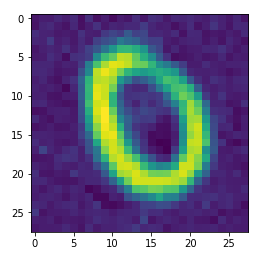
\includegraphics[width=0.4\textwidth]{autoenc1.png}
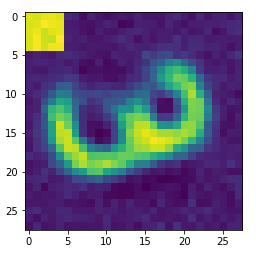
\includegraphics[width=0.4\textwidth]{autoenc2.png}
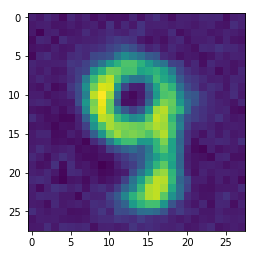
\includegraphics[width=0.4\textwidth]{autoenc4.png}
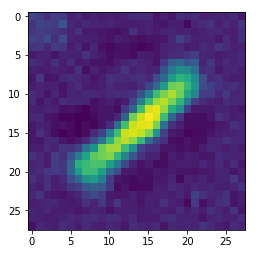
\includegraphics[width=0.4\textwidth]{autoenc6.png}
\caption{Reconstruction with Simple Autoencoder}
\label{fig:autorec}
\end{figure}

\section{Team members contribution}
\begin{itemize}
\item \textbf{Nikita Chizhov}: create experiments template, conducting experiments 
\item \textbf{Ekaterin Ivanova}: conducting experiments, presentation preparation, preparation of report
\item \textbf{Vadim Liventsev}: creation of the dataset, conducting experiments, presentation preparation 
\end{itemize}

\bibliographystyle{unsrt}
\bibliography{references}

\end{document}
